\subsection{PIPELINE CONSTRUCTION}\label{subsec:pipeline-construction}

Molecular ecological networks (MENs) represent biological interactions within microbial communities, where nodes symbolize molecular markers such as operational taxonomic units (OTUs), functional genes, or intergenic regions, and edges denote the interactions between them.
These networks are categorized into functional molecular ecological networks (fMENs), derived from functional gene markers, and phylogenetic molecular ecological networks (pMENs), based on phylogenetic gene markers.
\\\\
\noindent The process of Molecular Ecological Network Analysis (MENA) is divided into two primary phases.

\begin{figure}[H]
    \centering
    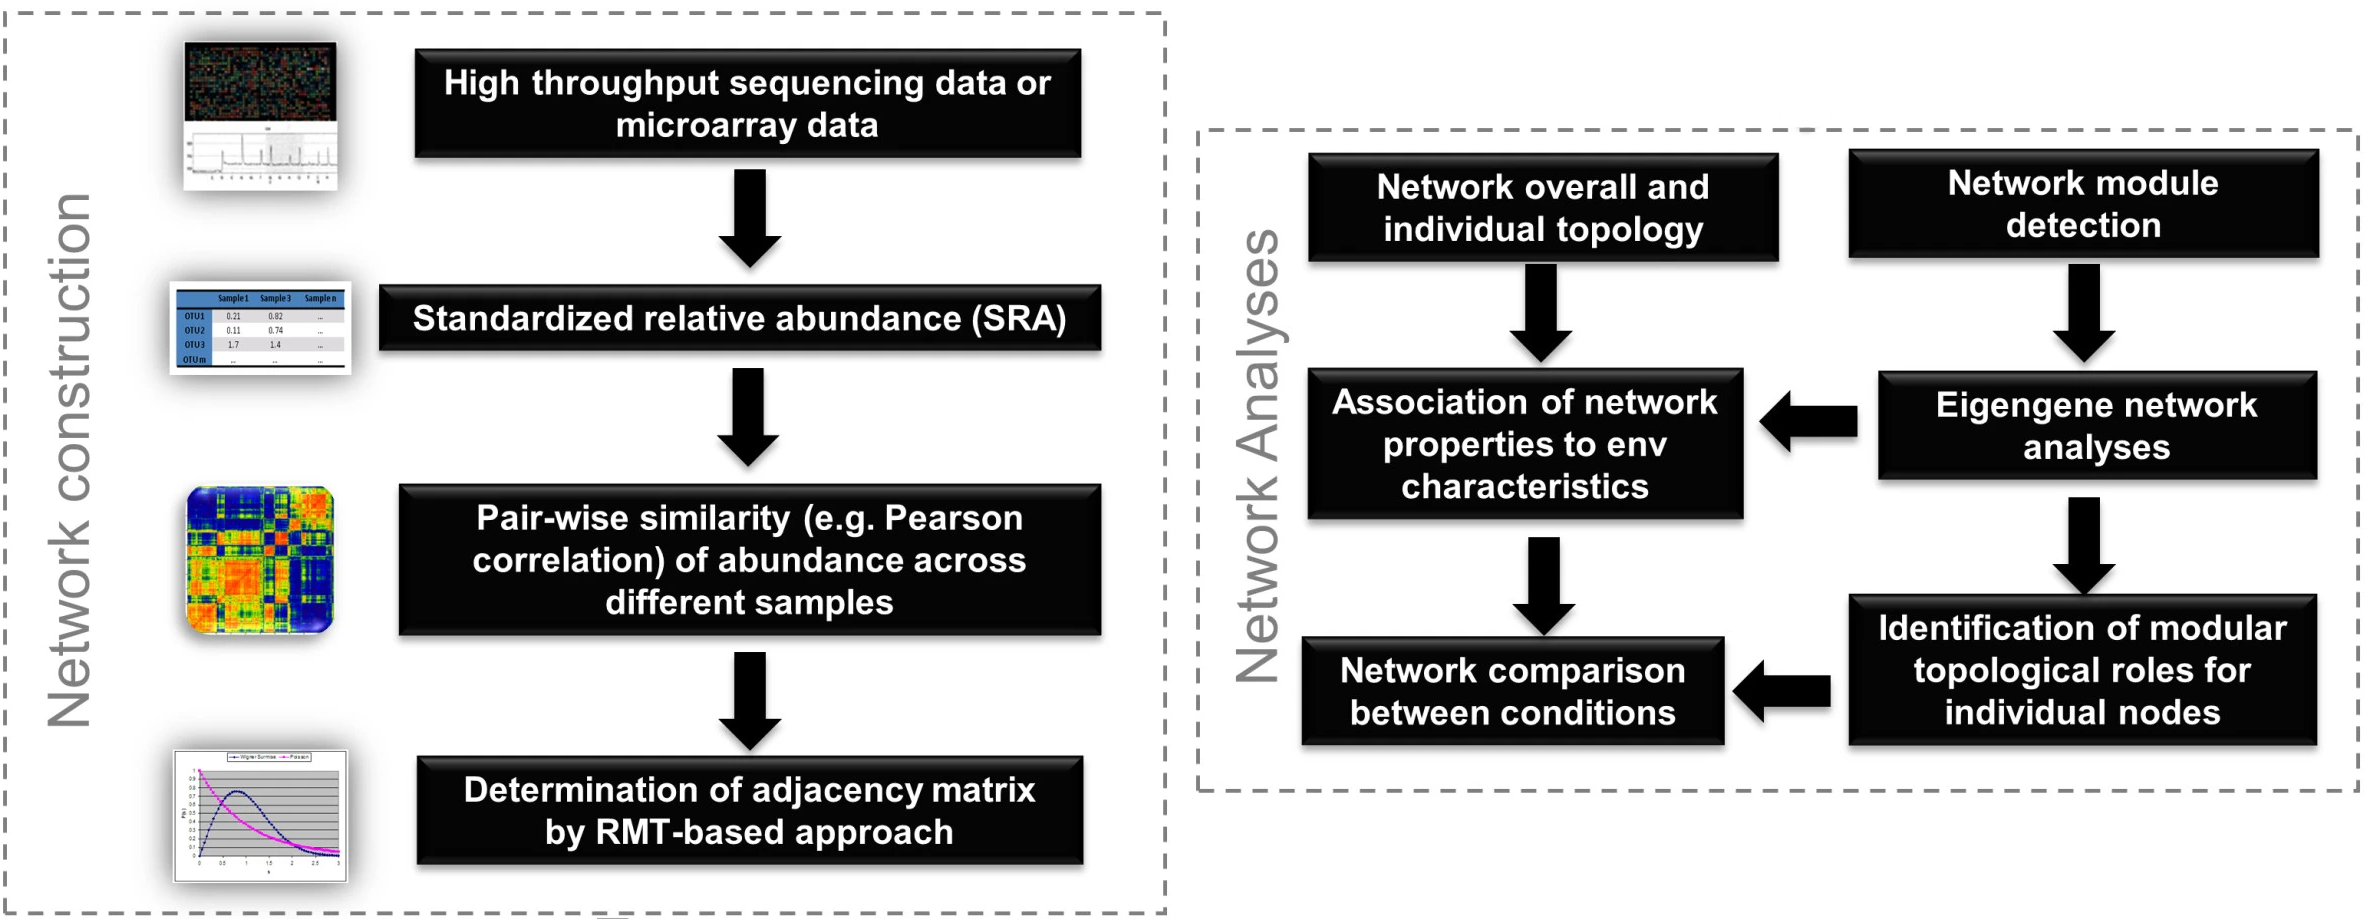
\includegraphics[width=1\textwidth]{Overview_of_the_Random_Matrix_Theory__RMT_-based_molecular_ecological_network_analysis_horizontal} % Path to your image file
    \caption{Overview of the Random Matrix Theory (RMT)-based molecular ecological network analysis\cite{deng_molecular_2012}}
    \label{fig:Overview_of_the_Random_Matrix_Theory__RMT_-based_molecular_ecological_network_analysis}
\end{figure}

The first phase(\autoref{fig:Overview_of_the_Random_Matrix_Theory__RMT_-based_molecular_ecological_network_analysis}) is network construction, which involves data collection of data then its transformation or standardization to normalize, calculation of pairwise similarity matrices, and the determination of the adjacency matrix using Random Matrix Theory.
The RMT-based approach is crucial for constructing an accurate network by defining an objective thresholds, resulting in an undirected network graph.

The second phase(\autoref{fig:Overview_of_the_Random_Matrix_Theory__RMT_-based_molecular_ecological_network_analysis}) is network analysis, which includes network topology characterization to evaluate the overall structure and properties of the network and the module detection to identify groups of tightly connected nodes known as modules.
Then a module-based eigengene analysis to understand underlying patterns and functions, and the identification of modular roles to determine the importance and function of nodes within modules.
An eigengene is a concept used in computational biology and bioinformatics to summarize the expression profiles of a group of co-expressed genes within a gene expression dataset.
Specifically, in the context of Weighted Gene Correlation Network Analysis (WGCNA), eigengenes serve as representative profiles for modules (clusters) of highly correlated genes or weighted combination of gene expressions that captures significant variation.
Additionally, eigengene network analysis explores higher-order organizational structures within the network, and associations between network properties and environmental characteristics are established to understand environmental influences.
Finally, comparative analysis evaluates network differences under varying conditions to assess how environmental changes affect network structure and interactions.
\\\\
Collectively, these methods enable researchers to uncover the complex interactions within microbial ecosystems, identify key functional populations at the OTU level, and understand how environmental factors influence these networks.

\newpage
\subsection{DETERMINATION OF THE ADJACENCY MATRIX USING \mbox{RANDOM} MATRIX THEORY}\label{subsec:determination-of-the-adjacency-matrix-using-random-matrix-theory}

RMT is used in MENA as a way to automatically identify thresholds for network construction(\autoref{fig:Process_of_random_matrix_theory-based_approach_for_automatically_detecting_threshold_to_construct_molecular_ecological_networks}).
It is able to do that by examining the statistical properties of matrices derived from high-throughput ecological data.

\begin{figure}[H]
    \centering
    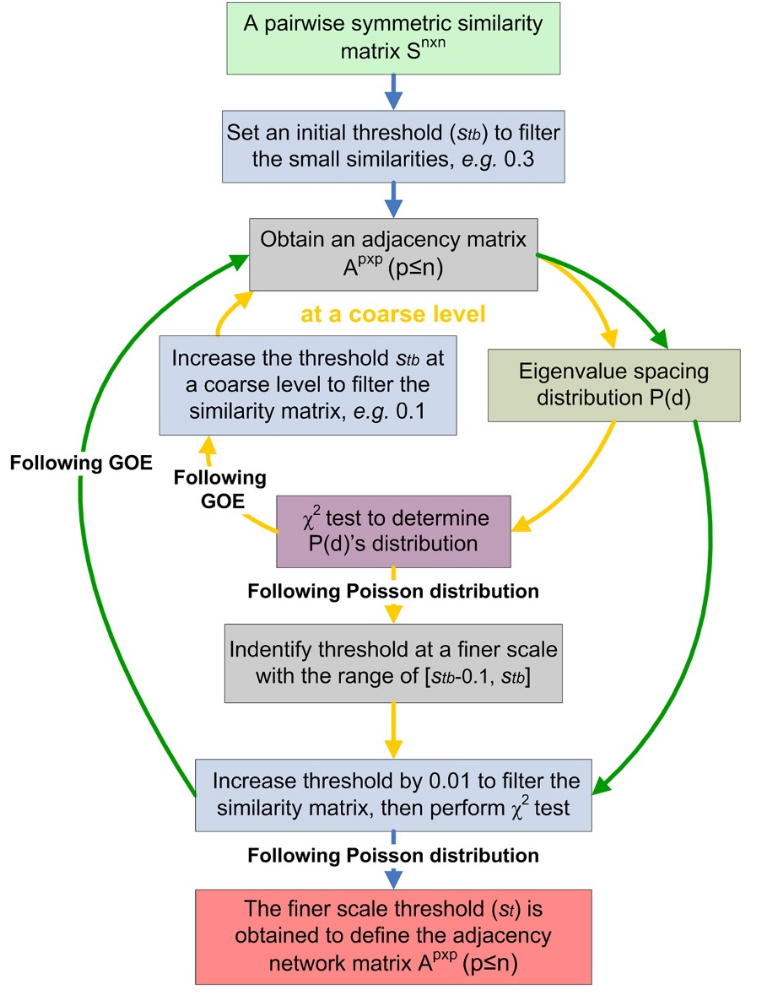
\includegraphics[width=0.72\textwidth]{Process of random matrix theory-based approach for automatically detecting threshold to construct molecular ecological networks} % Path to your image file
    \caption{Process of random matrix theory-based approach for automatically detecting a threshold to construct molecular ecological networks\cite{deng_molecular_2012}}
    \label{fig:Process_of_random_matrix_theory-based_approach_for_automatically_detecting_threshold_to_construct_molecular_ecological_networks}
\end{figure}

At first, the Pearson correlation matrix $R^{nxn}$ has to be computed using the standardized relative abundances of OTUs $X^{nxm}$, where $n$ is the number of distinct OTUs and $m$ is the number of samples.
This matrix $R^{nxn}$ is rapidly transformed into a similarity matrix $S^{nxn}$ by just taking the absolute values of $R^{nxn}$.
An adjacency matrix $A^{pxp}$, where p is the number of OTUs retained in the adjacency matrix with non-zero rows or columns, is then defined according to a threshold $s_{tb}$ set at first at 0.3.
The adjacency $a_{ij}$ between the i-th and j-th OTU is defined by thresholding the OTU abundance similarity:
\[a_{ij} =
\begin{cases}
s_{ij} & \text{if } s_{ij} \geq s_t, \\
0 & \text{if } s_{ij} < s_t.
\end{cases}\]
\\\\
\noindent The eigenvalues $\lambda_i$ of the adjacency matrix $A^{pxp}$ are then calculated.
Since it $A^{pxp}$ is a symmetric matrix, p eigenvalues can be obtained.
To test NNSD distribution, order the eigenvalues as $\lambda_1 \leq \lambda_2 \leq \ldots \leq \lambda_p$.
To unfold the eigenvalues, $\lambda_i$ is replaced by $e_i = N_{av}(\lambda_i)$ where $N_{av}$ is the continuous density of eigenvalues.
The continuous density $N_{av}$ can be obtained either by fitting the original integrated density to a cubic spline or by calculating the local average.
\\\\
The NNDS $P(s)$ is then calculated by taking the absolute value of the difference between consecutive eigenvalues.
This defines the probability density of unfolded eigenvalues spacing.
For the completely uncorrelated eigenvalues, P(d) follows Poisson statistic, and it can be expressed by, $P(s)=e^{-d}$ and the correlated eigenvalues, P(d) closely follow Wigner-Dyson distribution of the GOE statistics, and it can be expressed by $P(s) \approx \frac{\pi s}{2}e^{-\frac{\pi}{4}s^2}$(\autoref{fig:Wigner-Dyson_and_Poisson_distribution}).

\begin{figure}[H]
    \centering
    \includegraphics[width=1\textwidth]{Wigner’s surmise and Poisson} % Path to your image file
    \caption{Wigner-Dyson (blue) and Poisson (orange) distribution}
    \label{fig:Wigner-Dyson_and_Poisson_distribution}
\end{figure}

To determine whether the NNDS follows the Wigner-Dyson distribution or the Poisson distribution, the chi-squared test is used to fit it to the Poisson distribution.
By establishing the null hypothesis $H_0$ that $P(d)$ follows a Poisson distribution, the NNSD is tested to see if it conforms to this distribution.
If the NNSD does follow a Poisson distribution, then 0.1 is subtracted to the current threshold and then increases the threshold incrementally by 0.01 instead of 0.1.
This is tested by a $\chi^2$ defined like:
\[\chi^2=\sum \frac{d_i-E(d_i)}{E(d_i)}\]
With $d_i$ the observed nearest neighbor spacing and $E(d_i)$ the expected nearest neighbor spacing from Poisson distribution.

\noindent After determining the final threshold value $s_t$ at a finer scale, an adjacency matrix is constructed by retaining all OTUs with abundance similarity values exceeding the defined threshold.
Therefore, the final adjacency matrix will be defined like $A^{pxp}=[a_{ij}]$ is:

\[a_{ij} =
\begin{cases}
1 & \text{if } s_{ij} \geq s_t, \\
0 & \text{if } s_{ij} < s_t.
\end{cases}\]
\\\\
\noindent Here is a Python code snippet that demonstrates the process of determining the adjacency matrix using RMT.
It is assumed that the best threshold value $s_t$ has been reached, and the eigenvalues $\lambda_i$ of the adjacency matrix $A^{p \times p}$ are available.
\\\\
\begin{figure}[H] % H forces the figure to appear exactly here
\centering
\begin{lstlisting}[
    label={lst:pythoncode},
    language=Python,
    basicstyle=\fontsize{9pt}{13pt}\ttfamily, % Adjust font size and line spacing
]
import numpy as np
from scipy.interpolate import UnivariateSpline
from scipy.stats import chi2

# Generate sample eigenvalues for testing
N = 10000
lambdas = np.sort(np.random.normal(loc=0, scale=1, size=N))

N_lambda = np.arange(1, N + 1)  # Integrated density N(lambda_i) = i

# Create the spline with smoothing
spline = UnivariateSpline(lambdas, N_lambda, s=N, k=3)

# Compute N_av(lambda_i)
e_i = spline(lambdas)

# Compute the NNDS
s = np.diff(e_i)

# Khi^2 test, compute the expected spacings
x = np.linspace(0.5, 5, 50)
# Compute the histogram of spacings
p_s, bin_edges = np.histogram(s, bins=50, density=True)
s = 0.5 * (bin_edges[:-1] + bin_edges[1:])
poisson = np.exp(-s)

# Compute the chi-squared statistic
chi2_stat = np.sum((p_s - poisson) ** 2 / poisson)
print(f"{chi2_stat:.2f} < {chi2.ppf(0.99, 1):.2f} so H0 is accepted")
\end{lstlisting}
\caption{Python code for determining the adjacency matrix using RMT}
\label{fig:pythoncode}
\end{figure}

From this, it is concluded that "0.09 < 6.63 so H0 is accepted" indicating that the NNSD is consistent with the Poisson distribution~(\autoref{fig:Histogram_of_spacings_and_expected_spacings}).
This code snippet~(\autoref{fig:pythoncode}) demonstrates hwo easy the process of determining the adjacency matrix using RMT can be.
This simplicity mixed with the robustness of determining a threshold with RMT makes this method very elegant.
The histogram of spacings and the expected spacings can be plotted to visualize the results.

\begin{figure}[H]
    \centering
    \includegraphics[width=1\textwidth]{Wigner’s surmise and Poisson fitting P(s)} % Path to your image file
    \caption{Histogram of spacings and expected spacings}
    \label{fig:Histogram_of_spacings_and_expected_spacings}
\end{figure}

\noindent Thus, the adjacency matrix is constructed using the threshold $s_t$ determined by RMT, ensuring that the network is constructed objectively and consistently.

\subsection{COMPARISON TO LEGACY NETWORK METHODS AND ROBUSTNESS}\label{subsec:comparison-to-legacy-network-methods-and-robustness}

Both methodologies aim to understand relationships among biological entities, but they differ in principles, computational frameworks, and applications.
MENA uses advanced statistical tools like RMT to create robust, automated ecological networks.
In contrast, Legacy Co-Expression Network Analysis (LCNA) typically depends on co-expression thresholds to identify gene modules.
The table below compares these approaches, outlining their features, strengths, and limitations.
This comparison helps researchers choose the right method based on their research goals and data.

\begin{table}[H]
\centering
\renewcommand{\arraystretch}{1.5} % Adjusts row height
\begin{tabularx}{\textwidth}{@{}p{0.25\textwidth}X X@{}}
\toprule
\textbf{Feature} & \textbf{MENA} & \textbf{LCNA} \\
\midrule
\textbf{Network Construction Method} &
Uses Random Matrix Theory (RMT) for threshold determination, avoiding arbitrary cutoffs\cite{deng_molecular_2012} &
Relies on hard thresholding or predefined cutoff values, which can be subjective\cite{butte_discovering_2000} \\

\textbf{Robustness to Noise} &
Highly robust due to the RMT-based framework\cite{deng_molecular_2012} &
Sensitive to threshold selection and noise in data\cite{deng_molecular_2012} \\

\textbf{Topology Characteristics} &
Identifies scale-free, small-world, and modular networks\cite{deng_molecular_2012} &
Focuses on identifying clusters but may miss modular hierarchy\cite{horvath_analysis_2006} \\

\textbf{Key Applications} &
Analyzing ecological and environmental interactions, such as microbial community responses\cite{deng_molecular_2012} &
Studying biological processes like disease susceptibility and functional gene modules\cite{butte_discovering_2000,zhang_general_2005} \\

\textbf{Threshold Determination} &
Automated through RMT to ensure consistency\cite{deng_molecular_2012} &
Arbitrary or empirically determined, leading to potential biases\cite{deng_molecular_2012} \\

\textbf{Integration with Functional Data} &
Facilitates module-based eigengene analysis for deeper insights\cite{deng_molecular_2012} &
Limited integration with functional data without additional preprocessing\cite{chen_variations_2008} \\

\textbf{Software Availability} &
Supported by tools like MENAP for streamlined analysis\cite{deng_molecular_2012} &
Requires multiple tools or manual pipelines, such as clustering and visualization packages\cite{deng_molecular_2012} \\
\bottomrule
\end{tabularx}
\caption{Comparison of MENA and Legacy Co-Expression Network Analysis Methods}
\label{tab:mena_vs_lcna}
\end{table}

The comparison highlights the strengths and limitations of MENA and LCNA, helping to understand their optimal applications.
MENA uses Random Matrix Theory for automated thresholding, reducing subjective bias and enhancing robustness.
This makes it well-suited for high-throughput ecological studies where noise is a concern.
Its emphasis on modularity and eigengene analysis and also provides a better understanding of the network topology and environmental interactions, making it a great tool for microbial ecology and dynamic network studies.

\noindent In contrast, LCNA applies co-expression thresholds in a simpler framework, easily accessible when computational resources or specialized tools are limited.
However, its sensitivity to threshold selection and noise can lead to inconsistencies in network structure.
However, LCNA’s long-standing use and compatibility with diverse datasets have established it as a foundational method in network biology.
\\\\
Both approaches have distinct roles.
MENA excels in complex ecological data analysis, while LCNA offers a practical entry point for studying gene expression in simpler contexts.
Future developments may integrate MENA’s robustness with LCNA’s accessibility, creating a unified framework that overcomes their limitations.
Researchers should choose the method that best fits their dataset, goals, and computational expertise.

